\chapter{Initial Framework}
\label{Chapter4}
\lhead{Chapter 4. \emph{Initial Framework}}

\section{Overview}

The first phase of this work involved building a foundational prototype of a multi-agent clinical simulation using open-source language models. The system ran on a simple \texttt{while}-loop architecture that sequentially and naively routed requests between the Doctor, Patient, and Measurement agents. This functioned as the foundational control group, establishing the baseline sequential interaction paradigm that preceded the rigorous LangGraph state machine development. The main goal of this phase was to test whether relatively small, locally hosted LLMs (7B--8B parameters) could navigate a multi-turn diagnostic conversation and produce a recognisable disease prediction.

Figure~\ref{fig:agent-flowchart} illustrates the overall structure and information flow of the multi-agent clinical simulation framework. The diagram highlights how each agent interacts with the others through the Interaction Orchestrator, and how diagnostic reasoning emerges through sequential doctor--patient dialogue, structured test retrieval, and final moderator-based evaluation.

\begin{figure}[htbp]
    \centering
    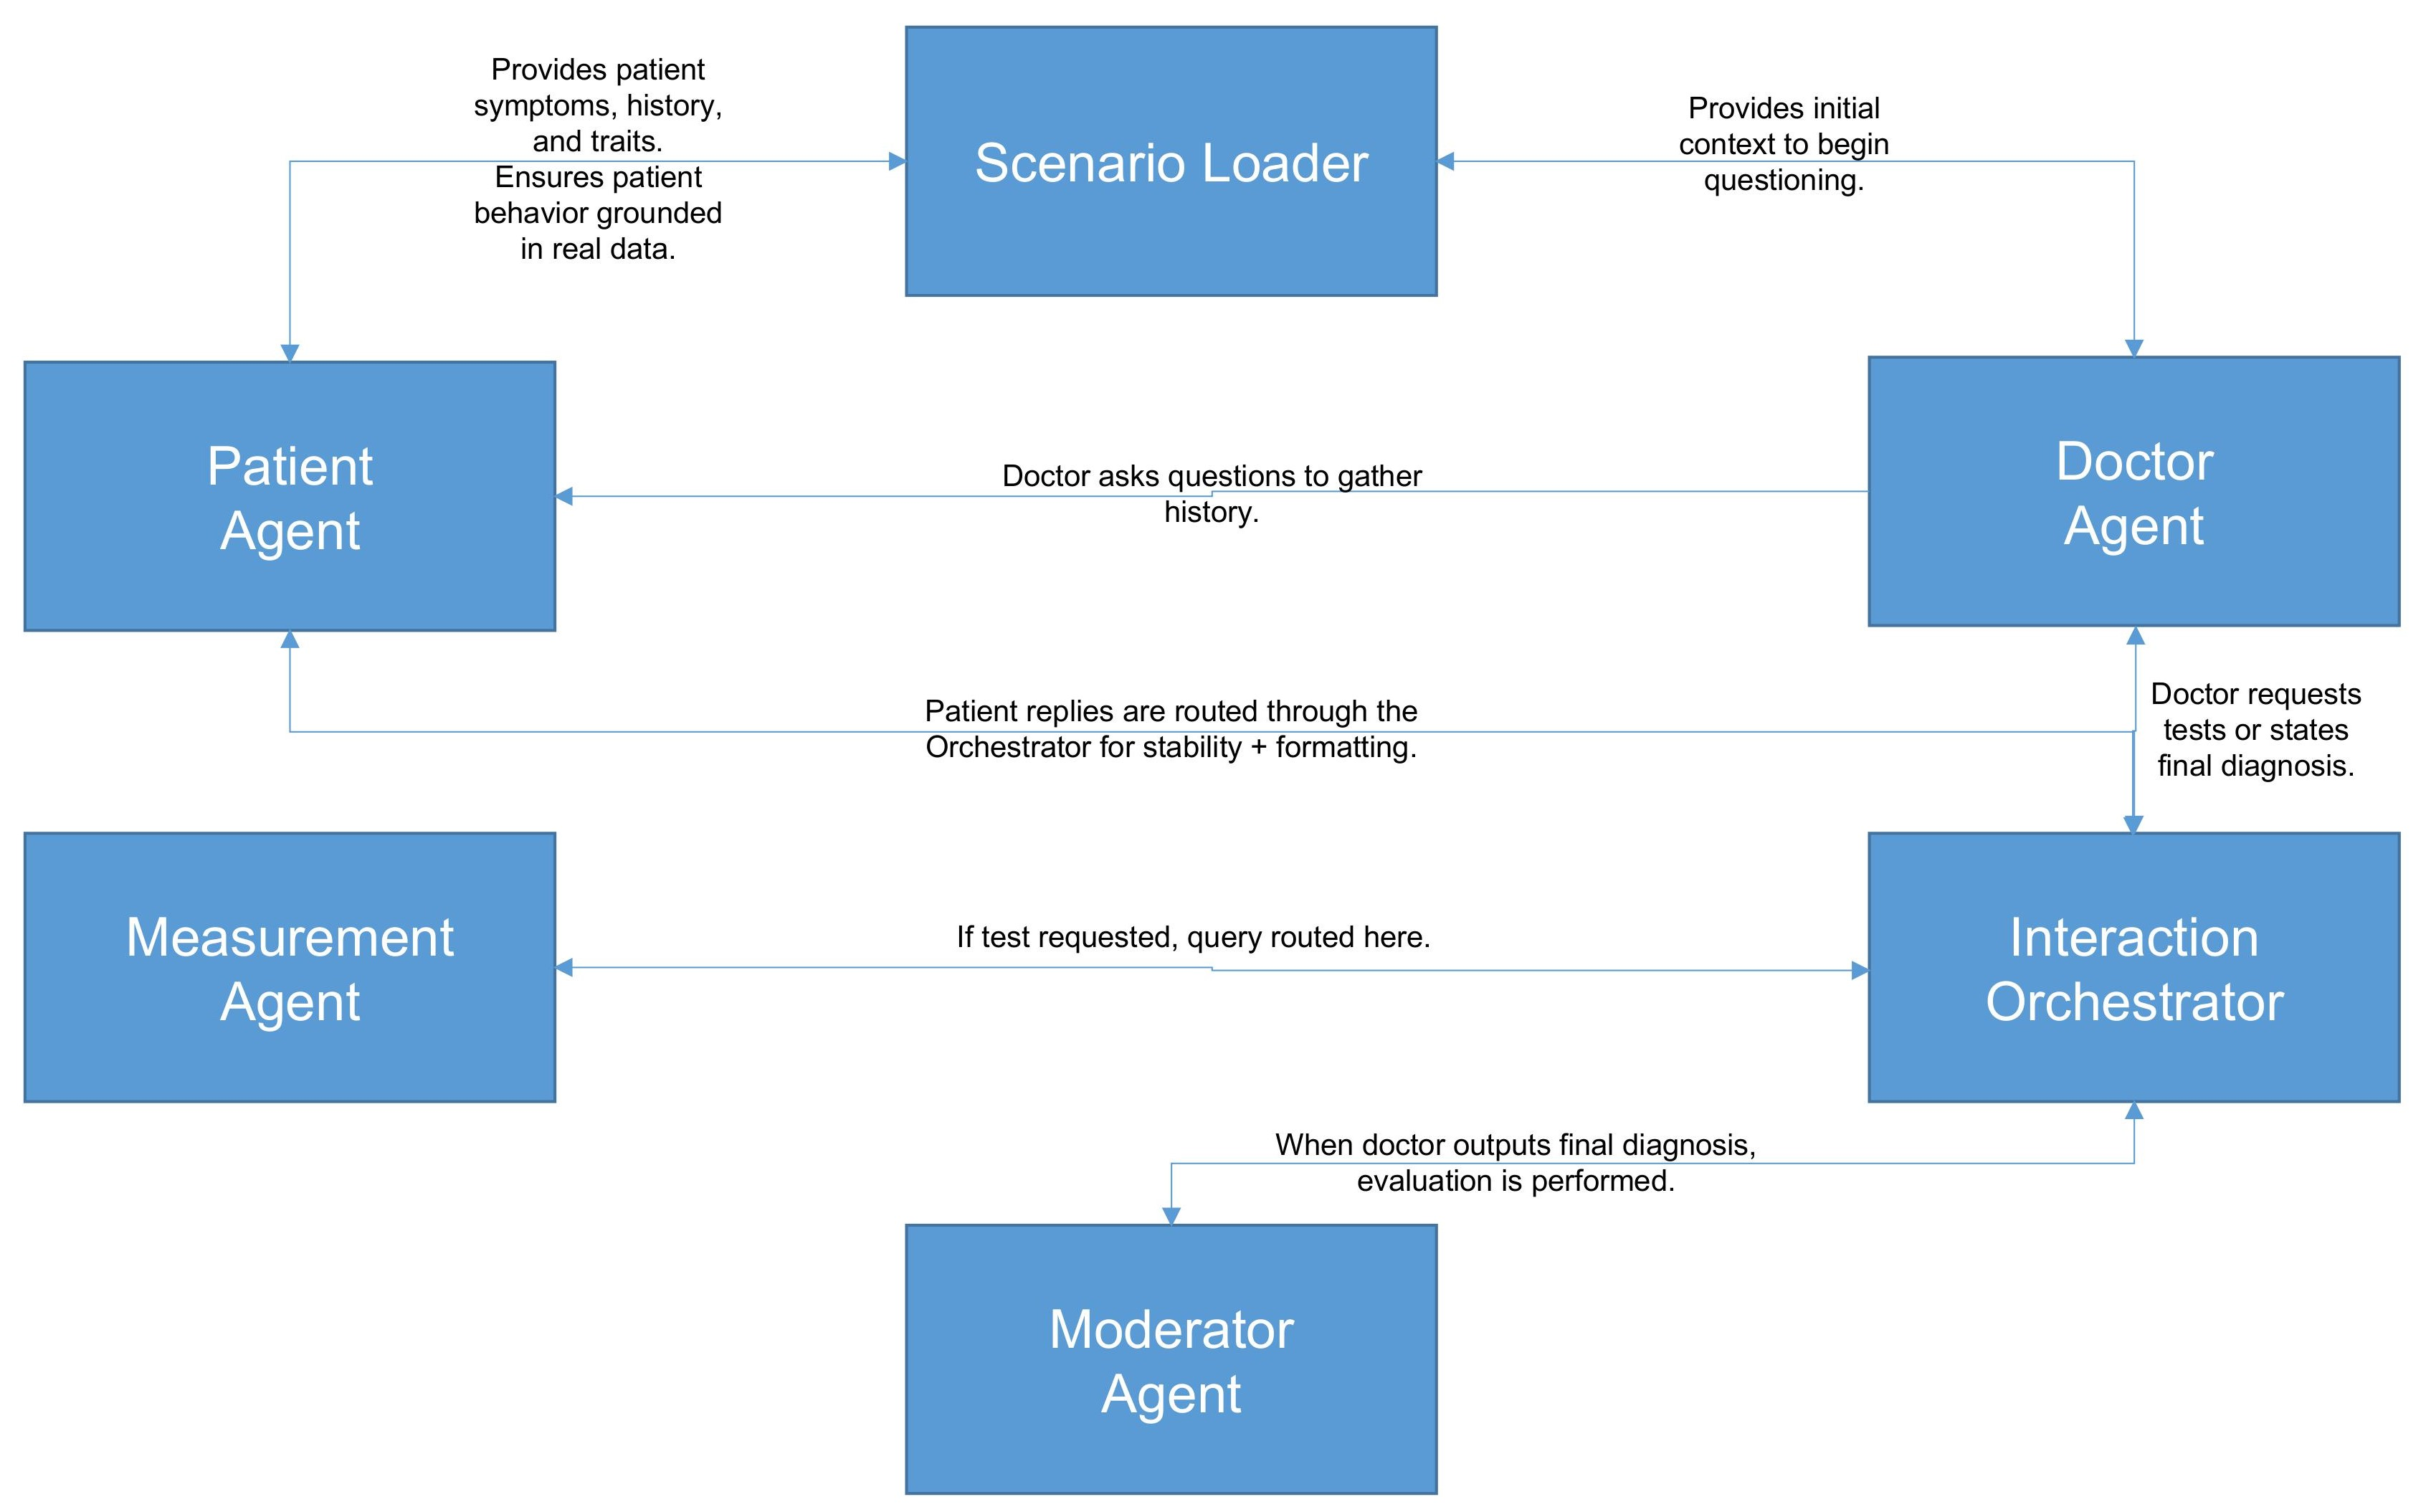
\includegraphics[width=\textwidth]{Pictures/Flowchart_pic.jpg}
    \caption{Overview of the multi-agent interaction workflow used in the clinical simulation framework. The Scenario Loader initializes each case and distributes case-specific information to the appropriate agents. The Doctor Agent performs history-taking, hypothesis generation, and test ordering. The Patient Agent produces symptom-grounded responses, while the Measurement Agent returns structured diagnostic tests upon request. All communication flows through the Interaction Orchestrator, which ensures turn-taking and state management. Once the Doctor provides a final diagnosis, the Moderator Agent evaluates its correctness through semantic comparison.}
    \label{fig:agent-flowchart}
\end{figure}

\section{Detailed Agent Definitions}

The initial loop coordinated the interactions of distinct agents, each implemented as a role-conditioned LLM:

\subsection{Doctor Agent}
The Doctor Agent is the primary reasoning engine being evaluated. Its objective is to gather information and form a diagnosis. It engages in:
\begin{itemize}
    \item History-taking and conversational follow-up questioning.
    \item Hypothesis formation and refinement.
    \item Ordering of diagnostic tests from the Measurement Agent.
    \item Synthesis of a final disease prediction.
\end{itemize}
To enforce programmatic extraction, the Doctor was strictly prompted to output \texttt{DIAGNOSIS\_READY: <diagnosis>} when concluding the test.

\subsection{Patient Agent}
The Patient Agent is a role-playing actor seeded with the OSCE scenario. To mimic realistic interactions, it:
\begin{itemize}
    \item Generates clinically grounded responses based strictly on the hidden scenario symptoms.
    \item Limits verbosity to 1--3 sentence conversational answers to prevent data dumping.
    \item Refrains from generating novel medical information outside the bounds of the provided case.
\end{itemize}

\subsection{Measurement Agent}
The Measurement Agent functions as a rigid lab interface. It supplies structured diagnostic data only upon explicit request. Supported modalities included:
\begin{itemize}
    \item Vital signs (temperature, blood pressure, heart rate).
    \item Laboratory test panels (complete blood count, metabolic panels).
    \item Imaging study text summaries.
    \item Physical examination findings (auscultation, palpation).
\end{itemize}

\subsection{Moderator Agent}
The Moderator Agent serves as the terminal evaluator. After the Doctor Agent emits a final diagnosis, the Moderator compares it against the hidden ground-truth label using semantic equivalence rather than exact string matching. It outputs a binary correctness flag (``Yes'' / ``No''), accommodating clinically valid synonyms and partial phrasing.

\subsection{Dialogue Orchestration}
A simple \texttt{while}-loop functioned as a basic orchestrator. It governed message routing and turn ordering, maintaining a shared raw text history to manage state transitions until the terminal diagnostic token was emitted.

\section{Evaluated Models}

Four open-source models were selected spanning a range from general-purpose instruction-tuning to narrow biomedical specialisation:
\begin{itemize}
    \item \textbf{Mistral-7B-Instruct-v0.2:} A strong general-purpose instruction-tuned model trained on diverse text corpora.
    \item \textbf{Microsoft BioGPT (1.5B):} A model pre-trained specifically on PubMed abstracts and biomedical literature.
    \item \textbf{JSL-Med-Sft-Llama-3-8B:} A Llama-3 derivative fine-tuned by John Snow Labs on clinical and biomedical datasets.
    \item \textbf{Apollo (7B):} A general-purpose baseline trained on broad web and text corpora without medical specialisation.
\end{itemize}

\section{Diagnostic Accuracy Results}

\subsection{Diagnostic Accuracy Calculation}

For each scenario, diagnostic correctness is determined by the Moderator Agent, which compares the Doctor Agent's final prediction against the ground truth. Overall accuracy is the ratio of correct diagnoses to total evaluated scenarios:
\begin{equation}
\text{Accuracy} = \frac{\text{Number of Correct Diagnoses}}{\text{Total Number of Scenarios}} \times 100
\end{equation}
This serves as the primary quantitative metric for the baseline framework.

\subsection{Model Performances}

Each model was tasked with diagnosing cases from the AgentClinic-MedQA subset. Table~\ref{tab:phase1_acc} and Figure~\ref{fig:phase1_acc} show the results.

\begin{table}[htbp]
\centering
\caption{Diagnostic accuracy of open-source LLMs on the AgentClinic-MedQA subset (initial framework).}
\label{tab:phase1_acc}
\begin{tabular}{@{}llc@{}}
\toprule
\textbf{Model} & \textbf{Training Data Alignment} & \textbf{Accuracy (\%)} \\ \midrule
Mistral-7B-Instruct-v0.2 & General instruction-tuning & 43.9 \\
Microsoft BioGPT         & Biomedical literature       & 34.6 \\
JSL-Med-Sft-Llama-3      & Clinical + Biomedical SFT   & 31.8 \\
Apollo                   & General text corpora        & 23.4 \\
\bottomrule
\end{tabular}
\end{table}

\begin{figure}[htbp]
\centering

\includegraphics[width=\textwidth]{Pictures/phase1_acc.pdf}
\caption{Baseline diagnostic accuracy of open-source LLMs in the initial simulation framework. Notably, the generalist Mistral-7B-Instruct-v0.2 outperformed all medically fine-tuned models.}
\label{fig:phase1_acc}
\end{figure}

Notably, the generalist Mistral-7B (43.9\%) outperformed all medically fine-tuned models, including BioGPT (34.6\%) and JSL-Med (31.8\%). This outcome is consistent with a known issue: \textit{catastrophic forgetting}. Medical fine-tuning datasets tend to be narrow in scope, and optimising for them erodes the broad conversational logic and instruction-following abilities that a multi-turn simulation demands. The result is degraded performance even when the model has superior declarative medical knowledge.

\section{Bias Impact Analysis}

Preliminary bias injections were run on the best-performing model (Mistral-7B, 43.9\% unbiased) to observe how performance held up under cognitive distortions:
\begin{itemize}
    \item \textbf{Recency bias (33.6\%)} causes noticeable degradation, suggesting that the model becomes overly influenced by recent cues rather than evaluating clinical evidence holistically.
    \item \textbf{Confirmation bias} leads to the lowest accuracy (31.8\%), indicating that once the model forms an early hypothesis, it tends to fixate on supporting evidence and ignore contradictory information.
\end{itemize}

The pattern was clear: cognitive biases systematically degrade diagnostic accuracy. Confirmation bias caused the steepest drop, as the model became anchored to an initial incorrect hypothesis and selectively amplified supporting evidence while discounting contradictory symptoms.

\section{Identified Architectural Limitations}

While the initial prototype worked, it had serious structural flaws. These motivated the complete system redesign:

\begin{enumerate}
    \item \textbf{Non-Deterministic Execution:} The \texttt{while}-loop frequently failed to handle agent transitions correctly when the LLM produced malformed stop tokens, causing simulation crashes or silent skips.
    \item \textbf{Absence of Trajectory Analysis:} Only terminal outcomes were measured. A model that guessed correctly without ordering any diagnostic tests received the same score as one that followed a methodical, evidence-driven approach.
    \item \textbf{Lexical Leakage Vulnerability:} Due to VRAM constraints, a homogeneous engine was used: the same Mistral-7B weights generated both the patient's symptoms and the doctor's diagnosis. It was observed that shared model weights cause both agents to project text into identical latent embedding manifolds. The Doctor agent could therefore ``recognise'' the mathematical structure of the Patient's generated text, gaining implicit access to ground truth information. This phenomenon is formalised as \textbf{Lexical Leakage}.
\end{enumerate}

These limitations motivated the development of the enhanced framework, described in the following chapter.
